\chapter{Simulation model}
\label{chap:simulation_model}

\section{General structure}

\subsection{Classes of the model}
The model is developed in Python and consists of two classes (see fig. \ref{uml}) : the HydropowerPlant class, which represents a run-of-the-river power plant and the Modelchain class which represents the simulation of one plant. The attributes and methods of each class are detailled in table \ref{att_meth}. \newline
A Modelchain object takes a HydropowerPlant object as input, as well as runoff time series. If attributes from the HydropowerPlant object are missing, the Modelchain object calculates them during initialization, through the extrapolation processes presented in subsection \ref{sub:assumptions}. The implementation of this process is detailed in subsections \ref{sub:check_feas} to \ref{sub:get_type}.
\begin{figure}[H]
\centering
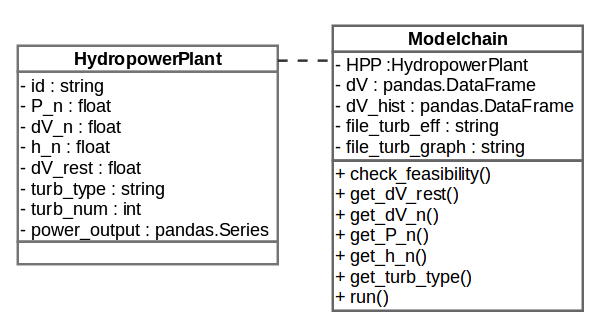
\includegraphics[width=12cm]{uml.png}
\caption{Classes of the hydropower model}
\label{uml}
\end{figure}

\begin{table}
\footnotesize
 \centering
 \caption{Attributes and methods of the classes}
 \label{att_meth}
 \begin{tabular}{|l|l|l|p{6cm}|}
  \cline{2-4}
  \multicolumn{1}{c|}{}&\multicolumn{3}{c|}{\textbf{class HydropowerPlant}}\\ \hline
  \multirow{8}{*}{\rotatebox[origin=c]{90}{\textbf{Attributes}}}&id&string&Identification of the plant\\
  &P{\_}n&float&Nominal power of the plant in \unit{W}\\
  &dV{\_}n&float&Nominal inflow of the plant in \unit{m\textsuperscript{3}\textperiodcentered s\textsuperscript{-1}}\\
  &h{\_}n&float&Nominal head of water in \unit{m}\\
  &dV{\_}rest&float&Residual water flow in \unit{m\textsuperscript{3}\textperiodcentered s\textsuperscript{-1}}\\
  &turb{\_}type&string&Type of turbine(s)\\
  &turb{\_}num&int&Number of turbines. Default : 1\\
  &power{\_}output&pandas.Series&Power output in \unit{W}\\
  \hline
  \multicolumn{4}{c}{}\\
  \cline{2-4}
  \multicolumn{1}{c|}{}&\multicolumn{3}{c|}{\textbf{class Modelchain}}\\ \hline
  \multirow{5}{*}[-1cm]{\rotatebox[origin=c]{90}{\textbf{Attributes}}}&HPP&HydropowerPlant&Plant to simulate\\
  &dV&pandas.DataFrame&Runoff time series in \unit{m\textsuperscript{3}\textperiodcentered s\textsuperscript{-1}} with DateTime index over the period to simulate\\
  &dV{\_}hist&pandas.DataFrame&Runoff time series in \unit{m\textsuperscript{3}\textperiodcentered s\textsuperscript{-1}} with DateTime index over several past years\\
  &file{\_}turb{\_}eff&string&File containing parameters about turbine efficiencies\\
  &file{\_}turb{\_}graph&string&File containing the characteristic diagrams\\
  \hline
  \multirow{7}[5]{*}{\rotatebox[origin=c]{90}{\textbf{Methods}}}&check{\_}feasibility()&boolean&Checks if input data is sufficient \\
  &get{\_}dV{\_}rest()&float&Calculates residual runoff in \unit{m\textsuperscript{3}\textperiodcentered s\textsuperscript{-1}}\\
  &get{\_}dV{\_}n()&float&Calculates nominal runoff in \unit{m\textsuperscript{3}\textperiodcentered s\textsuperscript{-1}}\\
  &get{\_}P{\_}n()&float&Calculates nominal power in \unit{W}\\
  &get{\_}h{\_}n()&float&Calculates nominal head in \unit{m}\\
  &get{\_}turb{\_}type()&string&Finds type of turbine\\
  &run{\_}model()&void&Calculates HPP.power{\_}output in \unit{W}\\
  \hline
 \end{tabular}
\end{table}

\subsection{Inputs and outputs}

The HydropowerPlant class has one compulsory parameter (id) and six optional parameters (P{\_}n, dV{\_}n, h{\_}n, dV{\_}rest, turb{\_}type, turb{\_}num). The number of turbines (turb{\_}num) is by default set to one when not filled in and the other optional parameters are extrapolated in the Modelchain class. \newline 
The Modelchain class takes pandas DataFrames as input for runoff. They can be read from csv files or extracted from a database, as presented in sections \ref{sub:ex_with_csv} and \ref{sub:ex_with_oedb}. These DataFrames require a DateTime index and a column named 'dV' containing runoff values. In order to correctly extrapolate the nominal water flow and the residual water flow from the historic values, DataFrame 'dV{\_}hist' has to cover many years (10 to 25 according to \cite{pacer} and \cite{cetmef}). Moreover, the time series should preferably be of whole years to avoid errors due to seasonal changes. \newline
The output power in \unit{W} is stored in the power{\_}output attribute of the HydropowerPlant object, as a pandas Series with the same DateTime index as the input 'dV' DataFrame.

\section{Implementation details}

\subsection{Initialization of Modelchain class}

When a Modelchain object is created, an initialization process takes place to check the integrity of the input and, if needs be, extrapolate the missing input data. The initialization process is presented in figure \ref{init} and the different methods are detailed in the following sections.

\begin{figure}[H]
\centering
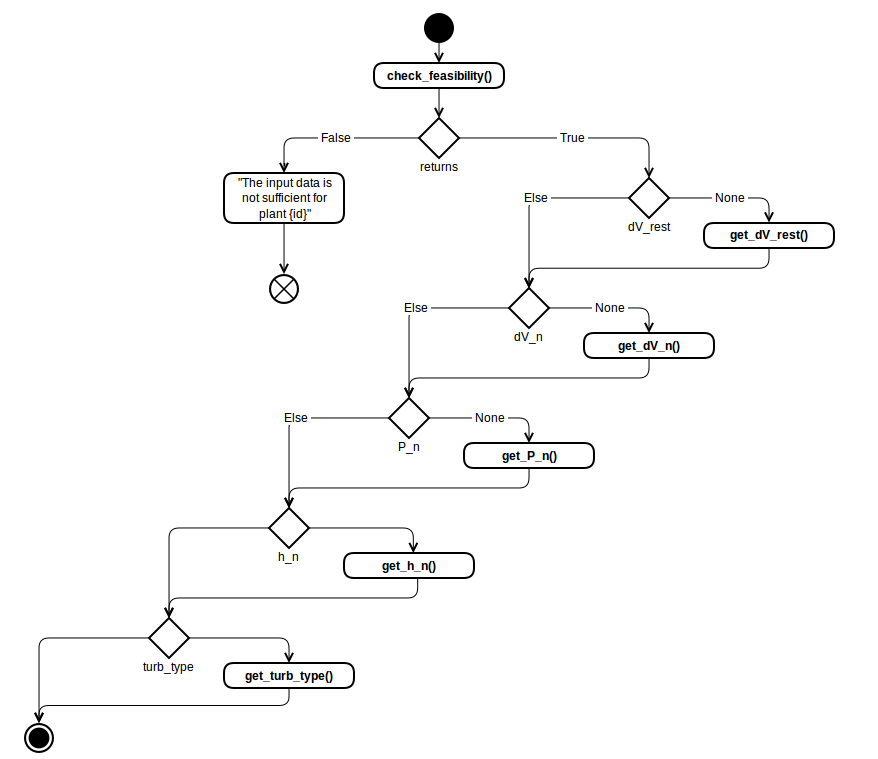
\includegraphics[width=15cm]{init.png}
\caption{Initialization of Modelchain class}
\label{init}
\end{figure}

\subsection{Method check{\_}feasibility()}
\label{sub:check_feas}

When a Modelchain object is initialized, the missing parameters of the HydropowerPlant object are extrapolated from the known parameters and the runoff history. For the extrapolation to be possible, enough parameters have to be filled in. With two parameters among  P{\_}n, dV{\_}n and h{\_}n can the third be calculated using the power equation in nominal operation (eq. \ref{eq_nom}) with nominal efficiencies of the generator and the turbine approximated to respectively \unit[95]{\%} and \unit[90]{\%}. If the runoff history is filled in, it can be use to extrapolate the nominal and residual water flows. If it is not filled in, the residual water flow can be set to 0 as it is very small part of the actual water flow. The type of turbine is then extrapolated from the nominal head and water flow.
\begin{equation}
\label{eq_nom} 
 P_\mathrm{n} = \rho_\mathrm{water} \cdot g \cdot \dot{V}_\mathrm{n} \cdot h_\mathrm{n} \cdot \eta_\mathrm{turbine, n} \cdot \eta_\mathrm{generator, n}
\end{equation}

Therefore, the first step of the initialization is to check the feasibility of the simulation. This is done with a logical test on the presence of inputs. The logical expression, obtained by filling in a Karnaugh map (see fig. \ref{karnaugh}), is given in equation \ref{eq_feas}.

\begin{equation}
\label{eq_feas} 
 Feasibility = (h_\mathrm{n} \land P_\mathrm{n}) \lor ((h_\mathrm{n} \lor P_\mathrm{n}) \land (\dot{V}_\mathrm{hist} \lor \dot{V}_\mathrm{n}))
\end{equation}

\begin{figure}[H]
\centering
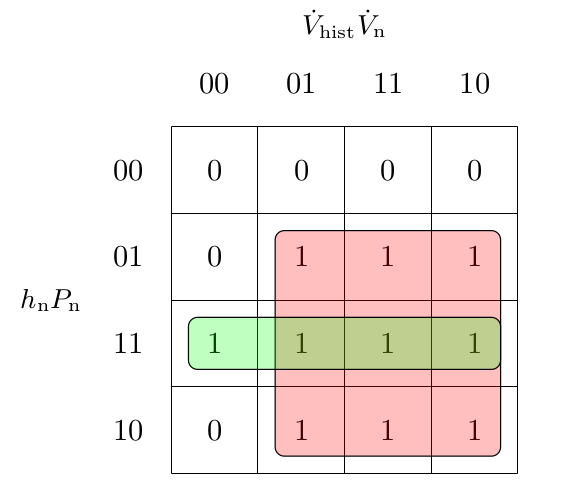
\includegraphics[width=8cm]{karnaugh.png}
\caption{Karnaugh map of simulation feasibility depending on inputs}
\label{karnaugh}
\end{figure}

\subsection{Method get{\_}dV{\_}rest()}
\label{sub:getdVrest}
The approach chosen to calculate the residual water flow is given in section \ref{sub:assumptions}. It is implemented in the model within the get{\_}dV{\_}rest() method of the Modelchain class, called during initialization.\newline If no runoff history has been specified, the residual water flow is set to zero. Otherwise, the ten most recent years of the runoff history are aggregated in a mean flow duration curve from which \.{V}\textsubscript{347} is extracted as the water flow attained or exceeded 347 days a year. The residual water flow \.{V}\textsubscript{rest} is then calculated following table \ref{res_wat} page \pageref{res_wat}. \newline
The python script of this method is given in appendix \ref{app:get_dV_rest}.

\subsection{Methods get{\_}dV{\_}n(), get{\_}h{\_}n() and get{\_}P{\_}n()}

If the nominal head and nominal power are given, the nominal water flow is calculated using equation \ref{eq_dV_n} with $\eta_\mathrm{turbine, n} = \unit[90]{\%}$ and $\eta_\mathrm{generator, n} = \unit[95]{\%}$. This same equation is used to calculate the nominal power or nominal head.

\begin{equation}
\label{eq_dV_n} 
 \dot{V}_\mathrm{n}=\frac{ P_\mathrm{n}}{\rho_\mathrm{water} \cdot g  \cdot h_\mathrm{n} \cdot \eta_\mathrm{turbine, n} \cdot \eta_\mathrm{generator, n}}
\end{equation}

If the nominal water flow cannot be obtained from equation \ref{eq_dV_n} because either the nominal head or the nominal power are missing, a history of water flows has to be specified for the simulation to be possible, and the nominal water flow is extrapolated from this history. The approach chosen to calculate the nominal water flow is given in section \ref{sub:assumptions}.\newline
The water flow history is sorted on runoff values and set with an index representing the percentage of time a value has been exceeded. The residual water flow is subtracted from this flow duration curve, to obtain a flow duration curve of usable runoff (see fig. \ref{fdc}). Finally, the nominal water flow is read as being the usable water flow reached \unit[20]{\%} of the time. \newline
The python script of this method is given in appendix \ref{app:get_dV_n}

\begin{figure}[H]
\centering
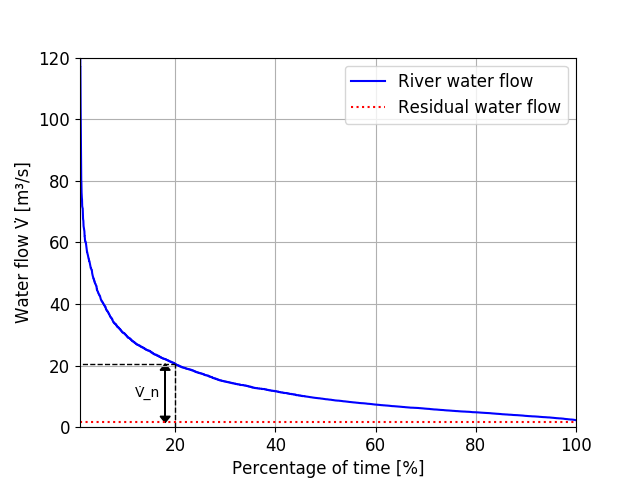
\includegraphics[width=12cm]{fdc.png}
\caption{Extrapolation of nominal water flow from the flow duration curve}
\label{fdc}
\end{figure}

\subsection{Method get{\_}turb{\_}type()}
\label{sub:get_type}

Once the residual water flow and the nominal water flow, head and power are set, the type of turbine can be worked out from locating the turbine on a h\textsubscript{n}/\.{V}\textsubscript{n} diagram such as the one shown on figure \ref{charac_diag} page \pageref{charac_diag}. \newline The implementation of this method in Python requires to be able of finding out if a point is inside a polygon. In that effect, a ray casting algorithm was used. Ray casting algorithms use the fact that a point is inside a polygon if a half-line starting from this point intersects the edges of the polygon an uneven number of times.\newline The intersection of half-lines with a polygon edges is not clear in the case where the origin of the half line is on an edge or vertex of the polygon. In our situation, this is automatically counted as being inside the polygon, and the ray casting algorithm is only used for points not locaed on the perimeter of the polygon. \newline To implement a ray casting algorithm in Python, the characteristic diagrams of each turbine type were stored in a csv file by the coordinates of their vertices (see appendix \ref{app:csv_vertices}), and a function to test the intersection of two segments was defined as follows : \newline
Segments [AD] and [BC] intersect $\iff 
\left\{
\begin{tabular}{@{}l@{}}
    A and D are on opposite sides of [BC] \\
    AND\\
    B and C are on opposite sides of [AD]
\end{tabular}\right.$\newline
A and D are on opposite sides of [BC] $\iff$ ccw(A,B,C) $\neq$ ccw(D,B,C) \cite{erickson} \newline \\
Where ccw(A,B,C) is a function testing whether A, B and C are in counterclockwise order. \newline  Therefore, testing in [AD] and [BC] intersect is equivalent to testing if only one and only one triplet among \{A,B,C\} and \{D,B,C\} is in counterclockwise order, and if one and only one triplet among \{B,A,D\} and \{C,A,D\} is in counterclockwise order.\newline \\
To test if a triplet \{A,B,C\} of non aligned points is in counterclockwise order, we compute the determinant of $\overrightarrow{AB}$ and $\overrightarrow{BC}$ :\newline
ccw(A,B,C) \tabto{2.5cm}$\iff \mathrm{det}(\overrightarrow{AB},\overrightarrow{AC})>0$\newline \\
\tabto{2.5cm}$\iff \begin{vmatrix}x_B-x_A&x_c-x_A\\y_B-y_A&y_c-y_A\end{vmatrix}>0$\newline\\
\tabto{2.5cm}$\iff (y_C-y_A)\cdot(x_B-x_A) > (y_B-y_A)\cdot(x_C-x_A)$ \newline
Where A, B and C are located by their abscissa x and ordinate y. \newline
\\
Having implemented these two functions in Python, the main function takes a horizontal ray starting in the point (dV\textsubscript{n},h\textsubscript{n}) representing the turbine to test and counts how many time it intersects the edges of each turbine type. When a turbine type gives a uneven number of intersections, the function stops and returns this type. Therefore, in the case of overlapping diagrams, the assigment is made to the first type tested, i.e. to the first type defined in the csv file. In the default file the order is as follows : first Kaplan, then Francis, then Pelton. If no results are found after testing all turbine types defined in the csv file, the function returns the type 'dummy', which represents a virtual turbine. The python script of this method is given in appendix \ref{app:get_turb_type}.

\subsection{Calculate power output}

Calling the run{\_}model() method of a Modelchain object calculates the electrical production time series of the plant and stores it in the power{\_}output attribute of the HydropowerPlant object. The run{\_}model() method calls an external function power{\_}output.run() which takes as inputs the HydropowerPlant object, the water flow in the turbine(s) \.{V}-\.{V}\textsubscript{rest} and the name of a csv file storing the parameters to calculate the turbine efficiency. If not specified otherwise, a default file is called using parameters from Quaschning \cite{quaschning} listed in table \ref{eff_param} page \ref{eff_param}, and specifying parameters for a ``dummy'' turbine type with a mean efficiency curve. The contents of the csv file are given in appendix \ref{app:csv_eff}. \newline
For each timestep of the inflow DataFrame, the load is calculated as $load = \frac{\dot{V}}{\dot{V}_\mathrm{n}}$, the efficiencies of the turbine and generator are calculated based on the values given in section \ref{eff_turb_gen} and an electric power value is calculated from equation \ref{eq_pow}. The flowchart of the function calculating power output is given in figure \ref{powout} and the script in appendix \ref{app:powout}.

\begin{equation}
  \label{eq_pow}
P= \left\{
    \begin{array}{ll}
	0 & \mbox{if load < turbine minimal load}\\
        P_\mathrm{n} & \mbox{if load}\geq 1 \\
        \eta_\mathrm{turbine} \cdot \eta_\mathrm{generator} \cdot \dot{V} \cdot h_\mathrm{n} \cdot g \cdot \rho & \mbox{otherwise}\\
    \end{array}
\right.
\end{equation}

\begin{figure}[H]
\centering
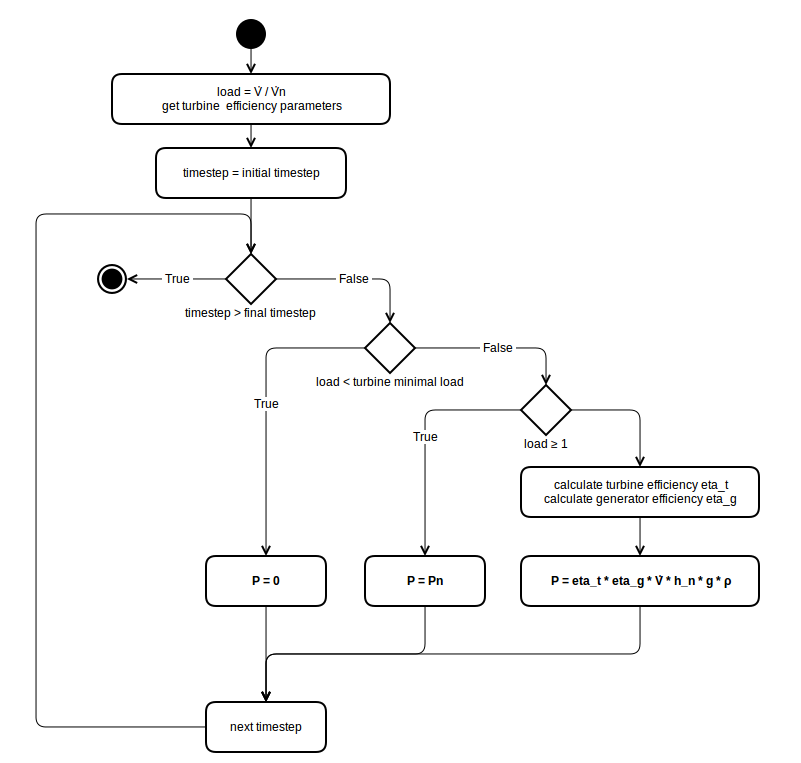
\includegraphics[width=12cm]{powout.png}
\caption{Flowchart of the function calculating the power output}
\label{powout}
\end{figure}



\section{Use examples}
Two use examples are provided with the model to help the user start simulations. Example \ref{sub:ex_with_csv} is designed for simulations with the user's own data (runoff and power plant parameters) and is the study case which results are presented in section \ref{sec:res_single}. Example \ref{sub:ex_with_oedb} is designed for simulations with the OpenEnergy Database and is the study case which results are presented in section  \ref{sec:res_th}.

\subsection{With csv files}
\label{sub:ex_with_csv}

This use example aims at simulating the production of a single power plant whose parameters are set by the user, with runoff time series imported from csv files. It is based on a power plant located in the french Vosges, on the Meurthe river. \newline
The first step is to read the runoff time series (historical and over the period to simulate) from csv files and store them into pandas DataFrames with a DateTime index and a column 'dV'.
In this example, the time series over the period to simulate have an hourly timestep and the historical time series have a daily timestep. An instance of the class HydropowerPlant is created, with user defined parameters, and taken as input in an instance of the class Modelchain, along with the runoff time series. \newline
After initialization, the plant parameters are displayed and the simulation can start by calling the run{\_}model() method. The example shows how the production from a single month can be extracted from the output and how the power output can be plotted as a function of time. \newline
The code of this example is given in appendix \ref{app:ex_with_csv}.

\subsection{With the OpenEnergy Database}
\label{sub:ex_with_oedb}

This use example aims at simulating the production of a region over a year, based on a register of run-of-the-river plants of the region, with runoff time series stored in a database. It is based on power plants of Thuringia and modeled runoff data from the WaterGAP software. The process would be similar with measured runoff data, as long as the database registers have been preprocessed following the guidelines of section \ref{sec:data_preproc}. \newline
The power plant register is imported from the OEDB via a SQL query and a database connection. It is stored in a DataFrame with the plant id, its electrical capacity and the id of the raster cell containing the runoff modeled data. The example iterates over each plant, fetches the available runoff time series from the database, creates HydropowerPlant and Modelchain instances, and stores the power output and parameters of each plant in a DataFrame. \newline
The example counts how many power plants were simulated and displays it, along with the total energy production. The dataframe of plants and power outputs can be exported as csv.\newline
The code of this example is given in appendix \ref{app:ex_with_oedb}.
